\chapter{Modèles de simulation et conditions aux limites}
\label{chap:modeles}


Dans le chapitre précédent, nous avons décrit un schéma 
Galerkin Discontinu (GD) semi-discret
\eqref{eq:formulation_semi-discrete} dont la convergence est assurée
par le théorème~\ref{thm:convergence_pb_discret}.
Ce schéma nous permettra de résoudre
les équations de Maxwell \eqref{eq:maxwell} dans un domaine borné donné.
Avant de poursuivre dans la description de l'implémentation discrète
que nous avons programmé de ce schéma, nous allons présenter les
principaux modèles physiques nécessaires à la résolution
des problèmes qui nous intéressent.
\\

Nous commençons par décrire des modèles correspondant à des conditions
de bord respectant la décroissance de l’énergie associée à la solution.
Décroissance requise afin de garantir l'unicité de la solution.
De telles conditions sont aussi nécessaires afin de limiter, informatiquement
parlant, la taille du problème. Car sans ces modèles, le rayon
du domaine de calcul devrait être supérieur à la distance parcourue
par une onde électromagnétique en autant de temps que le temps
physique simulé.
Nous présentons une technique permettant de résoudre un problème en domaine infini par l’ajout de couches absorbantes --- appelées PML pour
« \textit{Perfectly Matched Layer} » --- à la périphérie du domaine de calcul.

Dans un second temps, nous présentons des modèles représentant
de fines plaques de matériaux afin de nous permettre de remplacer
leur représentation géométrique en $3$ dimensions par de simples faces.
Nous verrons dans la suite (section \ref{ssect:stabilite_a_priori}) que la présence de ces mailles fines
produirait un malus important en temps de simulation. De plus,
de par leur nature, ils compliquent la phase de maillage.

Enfin, dans le but de traiter les matériaux diélectriques dont la
permittivité varie en fonction de la fréquence, nous décrivons
aussi un modèle volumique prenant en compte ces variations.
Ce type de modèle est intéressant dans le cas de simulations
faisant intervenir le corps humain qui présente ce type de matériaux.
\\

Ces modèles sont souvent similaires à ceux implémentés dans les
schémas de type différences finies d'un point de vue formel.
Une étude des conditions aux limites admissibles pour les équations
de Maxwell a été faite par Bourdel \textit{et al.}
\cite{Bourdel:1991:RNH:138062.138090}. Voir aussi \cite{fornet2012mathematical,crestetto:hal-00731021}.
\\



\section{Conditions aux limites}
\label{sect:conditions_aux_limites}


\subsection{Conducteur électrique parfait}
\label{ssect:PEC}


Cette condition de bord représente la présence d’un conducteur
électrique parfait (PEC pour « \textit{Perfect Electric Conductor} »).
Ce modèle correspond à un matériau de resistivité nulle (ou conductivité
infinie) et est généralement utilisé pour représenter les métaux
qui ont une resistivité proche de $0$.

Ce modèle est appliqué sur le bord du domaine de calcul
afin de simuler les ondes à l'intérieur d'une boîte métalique.
Il est aussi utilisé dans la modélisation des dispositifs
rayonnants, et permet de représenter un plan de masse ou tout autre
composant conducteur tel que les lignes microruban.
Physiquement, cette condition est donnée par :
\begin{align}
	\n \times \E = 0 ,
\end{align}
où $\n$ est le vecteur normal unitaire sortant à la maille considérée.

Soit $\MatPEC$ la matrice associée à cette condition.
Son noyau est l'ensemble $\ker (\MatPEC) = \lbrace \W = \Trp{(\Trp{\E}, \Trp{\H})} :
\n \times \E = 0 \rbrace$.
La condition d’existence \eqref{eq:thm_existence_unicite_2} de la solution
impose que cet ensemble soit de dimension $4$, ce qui est le cas ici :
l’annulation du champ électrique tangent est composé de deux contraintes.
La forme générique de la matrice $\MatPEC$ est donnée par :
\begin{align}
	\MatPEC =
	\begin{pmatrix}
		a (\n \times)^2 + b \n \times & 0 \\
		c (\n \times)^2 + d \n \times & 0
	\end{pmatrix}
\end{align}
où $a$, $b$, $c$ et $d$ sont des réels non tous nuls.

Pour une telle matrice $\MatPEC$, la condition de stabilité du théorème
\ref{thm:decroissance_energie} requiert la positivité de la matrice
$\frac{1}{2} \Aini + \MatPEC$, \textit{i.e.} :
\begin{equation}
	\begin{aligned}
		0 \le &\int_{\Bord{\PbEsp}}
			\left( \left( \frac{1}{2} \Aini + \MatPEC \right) \W \right)
			\cdot \W ds \\
		= &\int_{\Bord{\PbEsp}}
			\frac{1}{2} ((-\n \times \H) \cdot \E +
			(\n \times \E) \cdot \H) ds \\
		&+ \int_{\Bord{\PbEsp}}
			(a \n \times (\n \times \E) +
			 b \n \times \E) \cdot \E ds \\
		&+ \int_{\Bord{\PbEsp}}
			(c \n \times (\n \times \H) +
			 d \n \times \H) \cdot \E ds \\
		= &\int_{\Bord{\PbEsp}}
			a (\n \times (\n \times \E)) \cdot \E ds \\
		&+ \int_{\Bord{\PbEsp}}
			c (\n \times (\n \times \H)) \cdot \E ds \\
		&+ \int_{\Bord{\PbEsp}}
			(1 + d) (\n \times \H) \cdot \E ds .
	\end{aligned}
\end{equation}
Une condition suffisante pour que cette inégalité soit vraie est
que, pour tous champs $\E$ et $\H$ :
\begin{subequations}
	\begin{align}
		a (\n \times (\n \times \E)) \cdot \E &\ge 0 , \\
		c (\n \times (\n \times \H)) \cdot \E &\ge 0 , \\
		(1 + d) (\n \times \H) \cdot \E &\ge 0 .
	\end{align}
\end{subequations}
Cette condition est réalisée si $a \le 0$, $c = 0$ et $d = -1$.

Nous remarquerons que la valeur de $b$ n'a aucune incidence sur la
stabilité de cette condition de bord, nous pouvons donc choisir
$b = 0$ pour simplifier les calculs. De plus, le réel $a$
se révèle être un paramètre permettant de conditionner
la dissipation numérique de cette condition.

Les résultats obtenus au cours de la thèse de Strub \cite{strub:tel-01651258}
montrent que le choix du paramètre $a = -1$ augmente
la dissipation de ce modèle et ainsi améliore la stabilité
dans des cas où les mailles du maillage sont très déformées.
La matrice $\MatPEC$ s'écrit alors :
\begin{align}
	\MatPEC =
	\begin{pmatrix}
		- (\n \times)^2 & 0 \\
		- \n \times & 0
	\end{pmatrix} .
\end{align}


Cette formulation correspond donc à l'application d'un champ
fictif $\W^\star$, défini en fonction de $\W$,
imposé du côté extérieur à la maille :
\begin{align}
	\W^\star =
	\begin{pmatrix}
		\E^\top - \E^\bot \\
		\H^\bot - \H^\top 
	\end{pmatrix}
%	=
%	\begin{pmatrix}
%		\E - 2 (\n \cdot \E) \n \\
%		2 (\n \cdot \H) \n - \H
%	\end{pmatrix}
	,
\end{align}
où $\E^\bot$ et $\H^\bot$, respectivement $\E^\top$ et $\H^\top$,
sont les composantes orthogonales, respectivement tangentielles,
à la surface des champs $\E$ et $\H$.

Dans ce cas, le flux associé à cette condition s’écrit :
\begin{align}
	\FluxPEC{\W}{\n} = \Flux{\W}{\W^\star}{\n}
\end{align}
où $\F$ est le flux numérique décentré.
\\


\subsection{Conducteur magnétique parfait}
\label{ssect:PMC}

Dans la section précédente, nous avons présenté le modèle représentant la
condition de conducteur électrique parfait. En suivant le même raisonnement
nous pouvons définir une condition de bord représentant un conducteur
magnétique parfait (PMC).

Ce modèle peut être utilisé de manière combinée avec le PEC pour résoudre
des problèmes de propagation d'ondes planes dans un espace
de dimension $3$, notamment dans le but de tester d'autres
modèles de matériaux.

Physiquement, cette condition est donnée par :
\begin{align}
	\n \times \H = 0 ,
\end{align}
où $\n$ est le vecteur normal unitaire sortant à la maille considérée.
Nous obtenons alors la matrice correspondante, avec dissipation :
\begin{align}
	\MatPMC =
	\begin{pmatrix}
		0 & - (\n \times)^2 \\
		0 & - \n \times
	\end{pmatrix} .
\end{align}
\\

%\todo{écrire $\n \times \n \times$ ?}
% ou pas, je ne sais pas

\subsection{Condition d'impédance de surface}
\label{ssect:SIBC}


Cette condition de bord a initiallement été défini par Senior \cite{Senior1960} sous l'acronyme SIBC (pour
« \textit{Surface Impedance Boundary Condition} »).
Il s'agit d'une formulation générale dont nous présenterons
deux cas particuliers dans la suite : la condition de type Silver-Müller
et le modèle de Bérenger.

Le principe de cette condition est de lier les champs électrique et magnétique
tangents au bord du domaine par une relation faisant intervenir une
impédance de surface, notée $z \in \EnsR^{+}$.
Nous nous plaçons dans le cas où l’impédance ne dépend pas de la fréquence.

La formule associée à cette condition est connue sous le nom de
« relation de Léontovitch » :
\begin{align}
	\n \times \E + z \n \times (\n \times \H) = 0
	\label{eq:leontovitch} ,
\end{align}
où $\n$ est le vecteur normal unitaire sortant à la maille considérée.

En effectuant le produit vectoriel de cette équation par $\n$,
nous obtenons une formulation équivalente nous permettant de déduire
une matrice $\MatSIBC$ décrivant cette condition et donnée par :
\begin{align}
	\MatSIBC =
	\begin{pmatrix}
		a (\n \times)^2 & - a z \n \times \\
		b \n \times & b z (\n \times)^2
	\end{pmatrix}
\end{align}
où $a$ et $b$ sont des réels non tous deux nuls.


La condition d’existence \eqref{eq:thm_existence_unicite_2} est toujours
vérifiée pour une matrice de cette forme.
La condition de stabilité du théorème
\ref{thm:decroissance_energie} requiert la positivité de la matrice
$\Mat{B} = \frac{1}{2} \Aini + \MatSIBC$.
Soit $\W = \Trp{(\Trp{\E}, \Trp{\H})}$, alors :
\begin{equation}
	\begin{aligned}
		\Trp{\W} \Mat{B} \W
		= &(b + a z + 1) \H \cdot \n \times \E \\
		&+ a \E \cdot (\n \times (\n \times \E )) \\
		&+ b z \H \cdot (\n \times (\n \times \H )) .
	\end{aligned}
\end{equation}
Or, pour tout vecteur $\V \in \Esp$, la forme quadratique qui à
$\V$ associe $\V\cdot(\n\times(\n\times\V))$
est négative, en effet :
\begin{equation}
	\begin{aligned}
		\V \cdot (\n \times (\n \times \V))
		&= \V \cdot ((\n \cdot \V) \n
			- (\n \cdot \n) \V) \\
		&= (\n \cdot \V)^2 
			- (\n \cdot \n) (\V \cdot \V)
		\le 0
	\end{aligned}
\end{equation}
d’après l’inégalité de Cauchy-Schwartz.
Ainsi, la matrice $\Mat{B}$ est positive si $a$ et $b$ sont négatifs
et liés par la relation $b + a z + 1 = 0$.
Ce qui équivaut à :
\begin{subequations}
	\begin{align}
		- \frac{1}{z} \le a \le 0
		\label{eq:sibc_a} , \\
		b = - 1 - a z .
	\end{align}
\end{subequations}
Nous remarquons alors que la positivité de l’impédance $z$
est essentielle : dans le cas contraire la condition 
\eqref{eq:sibc_a} n'est jamais vérifiée.

La matrice $\MatSIBC$ s'écrit alors :
\begin{align}
	\MatSIBC =
	\begin{pmatrix}
		a (\n \times)^2 & - a z \n \times \\
		- (1 + a z) \n \times & - (1 + a z) z (\n \times)^2
	\end{pmatrix}
	\label{eq:mat_sibc} .
\end{align}
Le paramètre $a$ permet d'augmenter la dissipation numérique de cette condition
aux limites. Lorsqu’il est nul, la matrice $\Mat{B}$ est dégénérée et un
minimum d'énergie est dissipé.
\\

%  PH: il me semble que cette condition disspie toujours de l'énergie le paramètre a permet d'augmenter cette dissipation. à vérifier.
%  BW: reformulé

\subsection{Condition de Silver-Müller}
\label{ssect:silver_mueller}


La condition de Silver-Müller se traduit par l’application d’une condition
de radiation sur les bords du domaine.
Elle est un cas particulier de la condition
SIBC vue dans la section \ref{ssect:SIBC}
et a notamment été étudiée par Barucq \textit{et al.} \cite{barucq:hal-00925603}
et Bendali \textit{et al.} \cite{Bendali} et se traduit par une condition
aux limites de type SIBC avec une impédance de surface égale à celle du
vide, donnée par :
\begin{align}
	z_0 = \sqrt{\frac{\HPrm_0}{\EPrm_0}} .
\end{align}
Dans le cas des équations de Maxwell adimensionnées que nous
résoudrons dans le solveur implémenté,
l'impédance du vide est égale à $1$. Nous nous plaçons donc
dans ce cas afin de simplifier les écritures. 

En reprenant les résultats du modèle SIBC appliqué au cas particulier
que nous présentons ici, nous obtenons la matrice de condition
aux limites suivante :
\begin{align}
	\begin{pmatrix}
		a (\n \times)^2 & - a \n \times \\
		- (1 + a) \n \times & - (1 + a) (\n \times)^2
	\end{pmatrix} ,
\end{align}
avec $a$ le paramètre de dissipation tel que $-1 \le a \le 0$.

En choisissant $a = - \frac{1}{2}$, nous obtenons la matrice
$\MatSM = - \Neg{\Aini}$.
Dans ce cas, le flux associé à cette condition vaut :
\begin{align}
	\FluxSM{\W}{\n} = (\Aini + \MatSM) \W
	= \Pos{\Aini} \W .
\end{align}

Considérons maintenant une condition de Silver-Müller inhomogène.
Cette condition aux limites permet d’injecter dans le domaine
de calcul un champ incident que nous notons $\W_I$ :
\begin{align}
	\MatSM (\W - \W_I) = 0 .
\end{align}
Le flux associé à cette condition inhomogène s’exprime en fonction
du flux obtenu dans le cas homogène :
\begin{equation}
	\begin{aligned}
		\FluxSMI{\W}{\n} &= \FluxSM{\W}{\n} - \MatSM \W_I \\
		&= \Pos{\Aini} \W + \Neg{\Aini} \W_I \\
		&= \Flux{\W}{\W_I}{\n} .
	\end{aligned}
\end{equation}
Nous retrouvons ainsi le flux numérique décentré $\F$.
\\


\subsection{Condition limite absorbante}
\label{ssect:PML}

Pour calculer la solution des équations de Maxwell en espace libre, il est
nécessaire de simuler cet espace libre à l'aide d'une condition limite absorbante.
Sans une telle condition de bord, le domaine de calcul devrait être suffisamment
grand pour s'assurer qu'aucune onde réfléchie ne revienne polluer la scène électromagnétique
étudiée.

Le modèle Silver-Müller vu dans la section \ref{ssect:silver_mueller},
est connu pour sa facilité d'implémentation et son
faible coût de calcul. Cependant, ce modèle provoque des réflexions des ondes
sortantes contrairement au modèle PML couramment utilisé en
simulation électromagnétique.
\\


Le modèle PML a d'abord été introduit par Bérenger \cite{BERENGER1994185}
puis étendu et analysé théoriquement dans une vaste littérature
\cite{LASSAS2001739, laurens:tel-00475286, MAZET199859, MAZET2001599, 
LAHIVAARA20105144, Sullivan594858, Wrenger999615, Gedney546249, Fang556449}.
La construction de ce modèle utilise un changement de variables complexe effectué
sur la forme harmonique des équations de Maxwell. Ce modèle s'applique dans un
volume englobant le domaine de calcul et consiste en l'ajout d'une conductivité
électrique fictive qui a pour effet de dissiper les ondes électromagnétiques dans
la dimension imaginaire du modèle.
\\

%  PH: un dessin !
%  BW:
\begin{figure}[h]
	\begin{center}
		\caption{
			\label{img:domaine_PML}
			Représentation en $2$ dimensions du domaine $\PbEspPML$
			considéré, englobant le domaine de calcul $\PbEsp$.
		}
		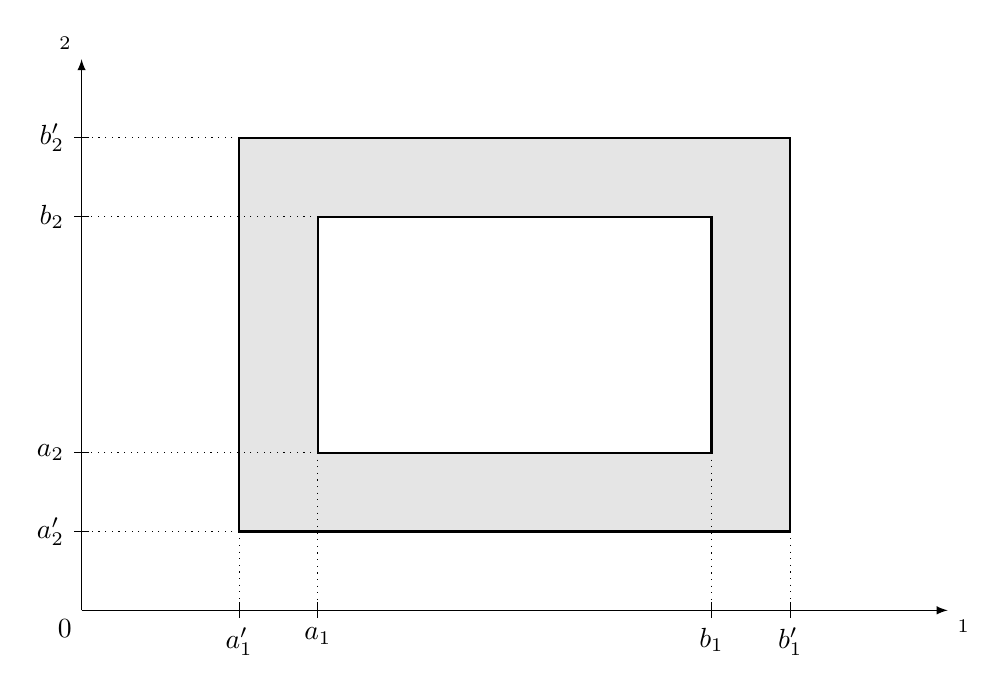
\begin{tikzpicture}[scale=1]
		\draw (0,0) node[below left] {$0$};
		\draw [arrows={-latex}] (0,0) -- (11,0); % axe x
		\draw (11,0) node[below right] {$\x_1$};
		\draw [arrows={-latex}] (0,0) -- (0,7); % axe y
		\draw (0,7) node[above left] {$\x_2$};
		\filldraw[thick,fill=gray!20,draw=black] (2,1) rectangle (9,6); % domaine pml
		\draw (5.5,5.5) node[] {$\PbEspPML$};
		\filldraw[thick,fill=white,draw=black] (3,2) rectangle (8,5); % domaine maxwell
		\draw (5.5,3.5) node[] {$\PbEsp$};
		\draw [dotted] (2,1) -- (2,0.1); % pointillés x min pml
		\draw [-] (2,0.1) -- (2,-0.1); % graduation
		\draw (2,-0.1) node[below] {$a'_1$};
		\draw [dotted] (3,2) -- (3,0.1); % pointillés x min maxwell
		\draw [-] (3,0.1) -- (3,-0.1); % graduation
		\draw (3,-0.1) node[below] {$a_1$};
		\draw [dotted] (8,2) -- (8,0.1); % pointillés x max maxwell
		\draw [-] (8,0.1) -- (8,-0.1); % graduation
		\draw (8,-0.1) node[below] {$b_1$};
		\draw [dotted] (9,1) -- (9,0.1); % pointillés x max pml
		\draw [-] (9,0.1) -- (9,-0.1); % graduation
		\draw (9,-0.1) node[below] {$b'_1$};
		\draw [dotted] (2,1) -- (0.1,1); % pointillés y min pml
		\draw [-] (0.1,1) -- (-0.1,1); % graduation
		\draw (-0.1,1) node[left] {$a'_2$};
		\draw [dotted] (3,2) -- (0.1,2); % pointillés y min maxwell
		\draw [-] (0.1,2) -- (-0.1,2); % graduation
		\draw (-0.1,2) node[left] {$a_2$};
		\draw [dotted] (3,5) -- (0.1,5); % pointillés y max maxwell
		\draw [-] (0.1,5) -- (-0.1,5); % graduation
		\draw (-0.1,5) node[left] {$b_2$};
		\draw [dotted] (2,6) -- (0.1,6); % pointillés y max pml
		\draw [-] (0.1,6) -- (-0.1,6); % graduation
		\draw (-0.1,6) node[left] {$b'_2$};
		\end{tikzpicture}
	\end{center}
\end{figure}

Considérons les équations de Maxwell dans le domaine de calcul $\PbEsp =
\ItvCC{a_1}{b_1} \times
\ItvCC{a_2}{b_2} \times
\ItvCC{a_3}{b_3}$ inclus dans $\Esp$.
Soit aussi le volume englobant $\PbEspPML =
\ItvCC{a'_1}{b'_1} \times
\ItvCC{a'_2}{b'_2} \times
\ItvCC{a'_3}{b'_3}$ défini tel que dans chaque
direction $a_i > a'_i$ et $b_i < b'_i$
(figure \ref{img:domaine_PML}).
Il est possible d’établir des modèles PML pour
des domaines de formes plus complexes comme par exemple
dans les travaux de Laurens \cite{laurens:tel-00475286}.


Dans le domaine $\PbEsp$, après transformée de Fourier-Laplace en temps du système
sans sources ($\ACnd = 0$ et $\Src = 0$), nous obtenons
l'expression fréquentielle des équations de Maxwell :
\begin{subequations} \label{eq:maxwell_f}
	\begin{align}
		p \EPrm \Ef - \Rot \Hf &= 0 , \\
		p \HPrm \Hf + \Rot \Ef &= 0 ,
	\end{align}
\end{subequations}
avec $p = j \omega$
où $j$ est la notation classique en physique du nombre complexe défini
tel que $j^2 = -1$, $\freq$ la fréquence et $\omega = 2 \pi \freq$ la pulsation.

\begin{remark}
	Le fait de considérer le système sans sources est légitime puisque nous nous situons
	en bordure de domaine de calcul où nous cherchons à simuler un espace libre infini.
\end{remark}


Nous introduisons le changement de variable complexe suivant
dans le domaine $\PbEspPML$ :
\begin{align}
	\tau(\x) = \hat{\x} :
	\hat{\x}_i = \x_i
	+ \frac{1}{p} \int_{0}^{\x_i}
	\ECnd_i (s) ds
	\label{eq:pml_chgt_var} ,
\end{align}
avec $\hat{\x}$ un point
de l'espace complexe $\EspC$ et $(\ECnd_i)_{i \in \Range{1}{3}}$
des fonctions réelles homogènes à des conductivités.
Cette opération se justifie théoriquement grâce à des outils avancés
de géométrie différentielle sur des variétés complexes décrits
dans les travaux de Lassas \textit{et al.} \cite{LASSAS2001739},
Laurens \cite{laurens:tel-00475286} et
Mazet \textit{et al.} \cite{MAZET199859}.

Remarquons que la matrice jacobienne $\tau'$ de $\tau$ est diagonale :
\begin{align}
	\tau' = \mathrm{diag} (s_1, s_2, s_3) ,
	\; \mathrm{avec} \;
	s_i = 1 + \frac{1}{p} \ECnd_i (\x_i) .
\end{align}
Les conductivités « fictives » $\ECnd_i$
sont supposées nulles sur $\PbEsp$ et de progression régulière sur
$\PbEspPML$ afin d'absorber progressivement les ondes sortantes
du domaine $\PbEsp$.
Un argument de type développement de Taylor, ou développement analytique,
permet de conclure que jusqu’à un certain ordre, la solution calculée
est bien la restriction à un domaine borné de la solution en milieu libre.

Nous exprimons aussi les opérateurs $\hat{\Ptl{i}}$
de dérivation complexe en fonction des opérateurs $\Ptl{i}$
en effectuant le changement de variable formel suivant :
%\todo{il manque $/s_i$, non ?}
\begin{align}
	\hat{\Ptl{i}} = \frac{1}{s_i} \Ptl{i} .
\end{align}
Nous pouvons alors exprimer les équations de Maxwell sur
$\PbEspPML$ avec les dérivées complexes formelles :
\begin{subequations} \label{eq:maxwell_f_c}
	\begin{align}
		p \EPrm \Ef - \RotC \Hf &= 0 , \\
		p \HPrm \Hf + \RotC \Ef &= 0 ,
	\end{align}
\end{subequations}
qui coïncide avec le système \eqref{eq:maxwell_f} sur $\PbEsp$.
En utilisant l’expression du rotationnel complexe d’un champ $\U$ :
\begin{align}
	\RotC \U =
	\Inv{\Jac{\tau}} \tau' (\Rot) \tau' \U ,
\end{align}
puis, en injectant cette formule dans le système de Maxwell complexe,
nous obtenons le système perturbé :
\begin{subequations} \label{eq:maxwell_f_p}
	\begin{align}
		p \EPrm \Jac{\tau} (\tau')^{-2} \Ef_s - \Rot \Hf_s &= 0 , \\
		p \HPrm \Jac{\tau} (\tau')^{-2} \Hf_s + \Rot \Ef_s &= 0 ,
	\end{align}
\end{subequations}
avec $\Ef_s = \tau' \Ef$ et $\Hf_s = \tau' \Hf$.

La matrice $\Jac{\tau} (\tau')^{-2}$ est une matrice diagonale :
\begin{align}
	\Jac{\tau} (\tau')^{-2} = 
	\mathrm{diag}\left(
		\frac{s_2 s_3}{s_1} ,
		\frac{s_3 s_1}{s_2} ,
		\frac{s_1 s_2}{s_3} 
	\right) .
\end{align}
Nous introduisons alors les matrices suivantes :
\begin{subequations}
	\begin{align}
		\Mat{\Sigma}_1 = \mathrm{diag} (
			\ECnd_1, \ECnd_2, \ECnd_3,
			\ECnd_1, \ECnd_2, \ECnd_3
		) , \\
		\Mat{\Sigma}_2 = \mathrm{diag} (
			\ECnd_2, \ECnd_3, \ECnd_1,
			\ECnd_2, \ECnd_3, \ECnd_1
		) , \\
		\Mat{\Sigma}_3 = \mathrm{diag} (
			\ECnd_3, \ECnd_1, \ECnd_2,
			\ECnd_3, \ECnd_1, \ECnd_2
		) ,
	\end{align}
\end{subequations}
et :
\begin{subequations}
	\begin{align}
		\Mat{S}_1 = \mathrm{diag} (
			s_1, s_2, s_3,
			s_1, s_2, s_3
		) , \\
		\Mat{S}_2 = \mathrm{diag} (
			s_2, s_3, s_1,
			s_2, s_3, s_1
		) , \\
		\Mat{S}_3 = \mathrm{diag} (
			s_3, s_1, s_2,
			s_3, s_1, s_2
		) ,
	\end{align}
\end{subequations}
telles que :
\begin{align}
	\Mat{S}_i = \Mat{I} + \frac{1}{p} \Mat{\Sigma}_i .
\end{align}
Nous pouvons alors écrire le système perturbé \eqref{eq:maxwell_f_p}
sous la forme :
\begin{align}
	p \At \Inv{(\Mat{S}_1)}
	\Mat{S}_2 \Mat{S}_3 \Wf_s
	+ \Aidi \Wf_s = 0
	\label{eq:maxwell_f_p_w} ,
\end{align}
avec $\Wf_s = \Trp{\left( \Trp{\Ef_s}, \Trp{\Hf_s}\right)}$.

En réécrivant la matrice du premier terme :
\begin{align}
	p \Inv{(\Mat{S}_1)} \Mat{S}_2 \Mat{S}_3 =
	\Inv{(p\Mat{I} + \Mat{\Sigma}_1)}
	(p\Mat{I} + \Mat{\Sigma}_2)
	(p\Mat{I} + \Mat{\Sigma}_3) ,
\end{align}
et puisque toutes ces matrices sont diagonales, nous pouvons réécrire ce produit
afin d'obtenir une décomposition en éléments simples, en raisonnant
sur un unique terme des diagonales. Ainsi, pour le
premier terme de chaque diagonale, nous obtenons :
\begin{equation}
	\begin{aligned}
		\Inv{(p + \ECnd_1)} &
		(p + \ECnd_2) (p + \ECnd_3)
		= \frac{(p + \ECnd_2) (p + \ECnd_3)}
			{p + \ECnd_1} \\
		&= \frac{p^2 + (\ECnd_2 + \ECnd_3) p + 
			\ECnd_2\ECnd_3}{p + \ECnd_1} \\
		&= p + \frac{(\ECnd_2 + \ECnd_3 - \ECnd_1) p 
			+ \ECnd_2\ECnd_3}{p + \ECnd_1} \\
		&= p + (\ECnd_2 + \ECnd_3 - \ECnd_1)
			+ \frac{-(\ECnd_2 + \ECnd_3 - \ECnd_1)
			\ECnd_1 + \ECnd_2\ECnd_3}{p + \ECnd_1} \\
		&= p + (\ECnd_2 + \ECnd_3 - \ECnd_1)
			+ \frac{\ECnd_1^2 - \ECnd_1 \ECnd_2 - \ECnd_1 \ECnd_3 + \ECnd_2\ECnd_3}{p + \ECnd_1} \\
		&= p + (\ECnd_2 + \ECnd_3 - \ECnd_1)
			+ \frac{(\ECnd_1 - \ECnd_2) (\ECnd_1 - \ECnd_3)}{p + \ECnd_1} ,
	\end{aligned}
\end{equation}
d'où, en raisonnant de manière analogue sur les autres
termes des diagonales :
\begin{align}
	p \Inv{(\Mat{S}_1)} \Mat{S}_2 \Mat{S}_3 =
	p \Mat{I} + \ACnd'
	+ \Mat{R}_1 \Inv{(p \Mat{I} + \Mat{\Sigma}_1)} \Mat{R}_2 ,
\end{align}
avec :
\begin{subequations}
	\begin{align}
		\ACnd' &=
		\Mat{\Sigma}_2 +
		\Mat{\Sigma}_3 -
		\Mat{\Sigma}_1 ,
		\\
		\Mat{R}_1 &=
		\Mat{\Sigma}_1 -
		\Mat{\Sigma}_2 ,
		\\
		\Mat{R}_2 &=
		\Mat{\Sigma}_1 -
		\Mat{\Sigma}_3 .
	\end{align}
\end{subequations}

Nous appliquons alors une transformée de Fourier-Laplace inverse au système
\eqref{eq:maxwell_f_p_w} et obtenons un système intégro-différentiel en temps.
Nous introduisons donc une variable intermédiaire $\V$ pour nous ramener
à un système d’EDP en espace-temps :
\begin{subequations}
	\begin{align}
		\At \Ptl{t} \W + \At \ACnd' \W + \At \Mat{R}_1 \V
		+ \Aidi \W &= 0 ,
		\\
		\Ptl{t} \V + \Mat{\Sigma}_1 \V
		- \Mat{R}_2 \W &= 0 .
	\end{align}
\end{subequations}
Ce système est un système de Friedrichs (définition \ref{def:friedrichs})
et s'écrit sous la forme :
\begin{align}
	\hat{\At} \Ptl{t} \hat{\W} + \hat{\ACnd} \hat{\W}
	+ \hat{\Ai} \Ptl{i} \hat{\W} = 0 , 
\end{align}
avec :
\begin{subequations}
	\begin{align}
		\hat{\W} &= \Trp{\left(
			\Trp{\W} , \Trp{\V} \right)} ,
		\\
		\hat{\At} &= \begin{pmatrix}
			\At & 0 \\
			0 & \Mat{I}
		\end{pmatrix} ,
		\\
		\hat{\ACnd} &= \begin{pmatrix}
			\At \ACnd' & \At \Mat{R}_1 \\
			- \Mat{R}_2 & \Mat{\Sigma}_1
		\end{pmatrix} ,
		\\
		\hat{\Ai} &= \begin{pmatrix}
			\Ai & 0 \\
			0 & 0
		\end{pmatrix} .
	\end{align}
\end{subequations}
L'intérêt de cette formulation est qu'elle est bien adaptée au solveur
que nous développons puisque ce dernier est en mesure de résoudre
tout système de Friedrichs.
\\

De manière générale, l'application du modèle PML au bord du domaine de calcul
s'effectue de manière régulière, en ajoutant des couches de mailles
d'épaisseur totale $\delta_{\max} = \Abs{a_i - a'_i} = \Abs{b_i - b'_i}$ dans chaque direction sur les
bords du domaine de calcul $\PbEsp$ (figure \ref{img:domaine_PML}).
Ces mailles adjointes forment le domaine englobant
$\PbEspPML$.

Le choix des conductivités fictives $\ECnd_i$ introduites
dans la construction du modèle PML \eqref{eq:pml_chgt_var} est fait
afin d'obtenir une certaine régularité dans l’absorption des ondes
sur le domaine $\PbEspPML$.
Cette régularité est importante pour assurer la « transparence » des PML.

Rappelons que ces conductivités sont nulles dans le domaine de calcul
$\PbEsp$. Dans le domaine $\PbEspPML$, elles sont
données par la formule :
\begin{align}
	\ECnd_i(\x_i) =
	\ECnd_{\max} \left(\frac{\delta_i(\x_i)}{\delta_{\max}}\right)^d
\end{align}
avec $\ECnd_{\max}$ la conductivité électrique maximale du modèle PML,
$d \in \EnsN$ la puissance du modèle dans la croissance des
conductivités, $\delta_{\max}$ l'épaisseur
du volume englobant et $\delta_i(\x_i)$ la distance de
$\x_i \in \PbEspPML$ au domaine Maxwell :
\begin{align}
	\delta_i(\x_i) =
	\begin{cases}
		a_i - \x_i &
			\mathrm{si} \; \x_i < a_i , \\
		\x_i - b_i &
			\mathrm{si} \; \x_i > b_i , \\
		0 & \mathrm{sinon} .
	\end{cases}
\end{align}

La conductivité maximale $\ECnd_{\max}$ est atteinte pour chaque
composante, dans sa direction associée,
uniquement aux bords du domaine $\PbEspPML$.
En général, nous utilisons ce modèle avec les paramètres suivants
qui génèrent un très faible taux de réflexion :
$d = 2$, $\ECnd_{\max} = 2000$ et $\delta_{\max} = \lambda / 2$,
avec $\lambda$ la longueur d'onde du signal, subdivisé
en $5$ couches de mailles hexaédriques.
%\todo{vérifier ces valeurs dans TETA}
La condition de bord appliquée à la frontière extérieure du
domaine $\PbEspPML$ est une condition
de conducteur électrique parfait présenté dans la section \ref{ssect:PEC}.
\\




\section{Modèles de plaques minces}
\label{sect:plaques_minces}

Les modèles de plaques minces sont utilisés en simulation numérique
afin de reproduire le comportement des matériaux de faible épaisseur.
Cela dans le but de supprimer du maillage les petites mailles
qui produiraient un malus important en temps de simulation
(section \ref{ssect:stabilite_a_priori}) et qui
compliquent fortement la phase de maillage.
Ces mailles fines sont alors remplacées par des faces sur lesquelles
un flux spécifique est appliqué.

La validité de ces modèles dépend de la fréquence de coupure $\freq_c$
des matériaux \eqref{eq:freq_coupure}. Nous avons déjà présenté un tel modèle dans la section
\ref{ssect:SIBC} : la condition limite d'impédance de surface SIBC.
Nous allons le présenter ici dans sa version dépendante de la fréquence.
Ce modèle est valide en hautes fréquences, pour des fréquences
supérieures à $20 \freq_c$.
Nous présentons deux autres modèles permettant de couvrir
une bande de fréquence plus étendue :
le modèle de plaque mince de Bérenger valide pour des fréquences inférieures
à la fréquence de coupure et le modèle BIBC valide sur la bande
de fréquences de $\freq_c / 10$ à $20 \freq_c$.
\\

\subsection{Plaque mince de Bérenger}
\label{ssect:berenger}

Le modèle de Bérenger \cite{berenger_thin_plane} permet de remplacer
efficacement les plaques minces de matériaux pour une fréquence
allant jusqu'à la fréquence de coupure $\freq_c$ de ce dernier.

Soit $S$ la surface représentant la plaque mince de matériau.
Cette surface est orientée par un vecteur normal unitaire $\n$,
dirigé de la maille $\L$ vers la maille $\R$.
Nous notons $\E_\L^\top$, respectivement
$\E_\R^\top$, la composante tangentielle à la surface $S$
du champ électrique du côté $\L$, respectivement $\R$.
Soient aussi $z_s$ et $z_t$ les impédances de surface et de
transfert de la plaque. Les champs électrique et magnétique
vérifient alors la relation de Léontovitch :
\begin{subequations}
	\begin{align} \label{eq:leontovich_transfert}
		\E_\L^\top + \n \times (z_s \H_\L + z_t \H_\R) &= 0 ,
		\\
		\E_\R^\top - \n \times (z_s \H_\R + z_t \H_\L) &= 0 .
	\end{align}
\end{subequations}

En prenant pour hypothèse que l’épaisseur de peau\footnote{L'épaisseur de la zone où se concentre le courant dans un conducteur, en surface.} est supérieure
à l’épaisseur de la plaque, nous pouvons approcher les impédances
de surface et de transfert par :
\begin{align}
	z_s = z_t = \frac{1}{\ECnd d} ,
\end{align}
avec $d$ l'épaisseur de la plaque et $\ECnd$ sa conductivité.
Cette approximation reste valide pour des fréquences inférieures
à la fréquence de coupure :
\begin{align}
	\freq_c = \frac{1}{2 \pi \HPrm \ECnd d^2}
	\label{eq:freq_coupure} .
\end{align}

Considérons dans un premier temps une plaque placée sur le bord
du domaine de calcul et munie d’une normale orientée vers l’extérieur.
En remarquant que :
\begin{align}
	\forall \V \in \Esp , \V^\top =
	- \n \times (\n \times \V) ,
\end{align}
la relation de Léontovitch précédente s'écrit :
\begin{align}
	\n \times (\n \times \E) - z_s \n \times \H = 0 .
\end{align}
Nous retrouvons alors la condition aux limites SIBC \eqref{eq:mat_sibc}
et nous en déduisons la matrice $\MatBER$
représentant la présente condition :
\begin{align}
	\MatBER =
	\begin{pmatrix}
		a (\n \times)^2 & - a z_s \n \times \\
		- (1 + a z_s) \n \times & - (1 + a z_s) z_s (\n \times)^2
	\end{pmatrix} .
\end{align}
La condition inhomogène s’écrit alors, pour un champ incident $\W_I$ :
\begin{equation}
	\begin{aligned}
		0 &= \MatBER (\W - \W_I) \\
		&= \begin{pmatrix}
			a \left( (\n \times)^2 (\E - \E_I)
				- z_s \n \times (\H - \H_I) \right) \\
			- (1 + a z_s) \left( \n \times (\E - \E_I)
				+ z_s (\n \times)^2 (\H - \H_I) \right)
		\end{pmatrix} ,
	\end{aligned}
\end{equation}
avec
$\W_I = \Trp{\left( \Trp{\E_I}, \Trp{\H_I} \right)}$.

Nous pouvons alors choisir le paramètre $a$ assurant la stabilité du
schéma :
\begin{align}
	- \frac{1}{z_s} \le a \le 0 .
\end{align}
Par exemple, en prenant $a = 0$, nous obtenons un flux non
dissipatif associé au modèle de Bérenger :
\begin{equation}
	\begin{aligned}
	\FluxBER{\W_\L}{\W_\R}{\n} &=
		\Aini \W_\L + \MatBER (\W_\L - \W_\R) \\
		&= \begin{pmatrix}
			- \n \times \H_\L \\
			\n \times \E_\R + z_s (\n \times)^2 (\H_\R - \H_\L)
		\end{pmatrix}.
	\end{aligned}
\end{equation}
Il est également possible d’ajouter une dissipation numérique dans le but de
stabiliser le schéma en prenant $a$ non nul.
\\

\subsection{Impédance de surface}
\label{ssect:SIBC_plaque}


Nous avons vu le modèle SIBC comme condition de bord dans la section
\ref{ssect:SIBC}. Ce modèle peut être implémenté pour prendre en compte
une impédance de surface variable en fonction de la fréquence.

Pour cela, nous utilisons la technique du \textit{vector fitting} \cite{772353}
dans le but d'approcher l'impédance de surface par une somme de fractions
rationnelles dans le domain fréquentiel :
\begin{align}
	z_s (\omega) = z_s^\infty \left( 1 +
	\sum_{k = 1}^{N_p} \frac{r_k}{j \omega - p_k} \right)
	\label{eq:impedance_surface_vf} ,
\end{align}
avec $z_s^\infty$ l'impédance de surface à la fréquence infinie,
$N_p$ le nombre de pôles, $p_k \in \EnsR$
les pôles et $r_k \in \EnsR$ les résidus.

Cette approximation est alors injectée dans la relation de Léontovitch
\eqref{eq:leontovitch} et nous obtenons le modèle SIBC de la section
\ref{ssect:SIBC} appliqué avec l'impédance à l'infini $z_s^\infty$, auquel
nous ajoutons $N_p$ courants annexes :
\begin{align}
	\tilde{\J}_k =  \frac{r_k}{j \omega - p_k} \Hf_\L ,
	\; \mathrm{pour} \; k \in \Range{1}{N_p} .
\end{align}
Ces courants s'appliquent uniquement du côté considéré de la plaque,
l'impédance de transfert étant nulle dans ce cas.

En revenant dans le domaine temporel en appliquant une transformée de Fourier-Laplace
inverse, nous obtenons $N_p$ équations différentielles ordinaires annexes,
pour $k \in \Range{1}{N_p}$ :
\begin{subequations}
	\begin{align}
		\Ptl{t} \J_k - p_k \J_k - r_k \H_\L &= 0 , \\
		\J_k(\x, 0) &= 0 .
	\end{align}
\end{subequations}
Ainsi, les champs $\W_\L = \Trp{(\Trp{\E_\L},\Trp{\H_\L})}$
vérifient le système :
\begin{subequations}
	\begin{align}
	\n \times (\n \times \E_\L) - z_s^\infty \n \times \H_\L &=
	z_s^\infty \n \times \sum_{k = 1}^{N_p} \J_k , \\
	\Ptl{t} \J_k - p_k \J_k - r_k \H_\L &= 0 ,
	\; \mathrm{pour} \; k \in \Range{1}{N_p} .
	\end{align}
\end{subequations}

Nous pouvons alors définir le flux SIBC à partir du flux de Bérenger
inhomogène pour l'impédance $z_s^\infty$ :
\begin{align}
	\FluxSIBC{\W_\L}{\n} = 
	\FluxBER{\W_\L}{\begin{pmatrix}
		0_{\Esp} \\
		- \sum_{k = 1}^{N_p} \J_k
		\end{pmatrix}}{\n} .
\end{align}
\\



\subsection{Impédance de surface bilatérale}
\label{ssect:bibc}

Le modèle d'impédance de surface bilatérale (ou BIBC pour
« \textit{Bilateral Impedance Boundary Condition} »)
est un modèle de SIBC pour lequel l'impédance de transfert n'est pas nulle.
Nous utilisons donc là aussi la technique du \textit{vector fitting} \cite{772353}
dans le but d'approcher les impédances de surface et de transfert
par une somme de fractions
rationnelles dans le domain fréquentiel :
\begin{subequations}
\begin{align}
z_s (\omega) &= z_s^\infty \left( 1 +
\sum_{k = 1}^{N_p} \frac{r_k}{j \omega - p_k} \right) , \\
z_t (\omega) &= z_t^\infty \left( 1 +
\sum_{k = 1}^{N'_p} \frac{r'_k}{j \omega - p'_k} \right)
\label{eq:impedance_surface_transfert_vf} ,
\end{align}
\end{subequations}
avec $z_s^\infty$ l'impédance de surface à la fréquence infinie,
$z_t^\infty$ l'impédance de transfert à la fréquence infinie,
$N_p$ et $N'_p$ le nombre de pôles pour chaque approximation, $p_k, p'_k \in \EnsR$
les pôles et $r_k, r'_k \in \EnsR$ les résidus.

Ces approximations sont injectées dans la relation de Léontovitch
\eqref{eq:leontovich_transfert} pour obtenir les
$N_p + N'_p$ courants annexes :
\begin{align}
\tilde{\J}_k =  \frac{r_k}{j \omega - p_k} \Hf_\L ,
\; \mathrm{pour} \; k \in \Range{1}{N_p} 
\end{align}
et
\begin{align}
\tilde{\J}'_k =  \frac{r'_k}{j \omega - p'_k} \Hf_\R ,
\; \mathrm{pour} \; k \in \Range{1}{N'_p} .
\end{align}

En revenant dans le domaine temporel en appliquant une transformée de Fourier-Laplace
inverse, nous obtenons $N_p + N'_p$ équations différentielles ordinaires annexes,
pour $k \in \Range{1}{N_p}$ :
\begin{subequations}
	\begin{align}
	\Ptl{t} \J_k - p_k \J_k - r_k \H_\L &= 0 , \\
	\J_k(\x, 0) &= 0 ,
	\end{align}
\end{subequations}
et pour $k \in \Range{1}{N'_p}$
\begin{subequations}
	\begin{align}
	\Ptl{t} \J'_k - p'_k \J'_k - r'_k \H_\R &= 0 , \\
	\J'_k(\x, 0) &= 0 .
	\end{align}
\end{subequations}
Ainsi, les champs $\W_\L = \Trp{(\Trp{\E_\L},\Trp{\H_\L})}$
et $\W_\R = \Trp{(\Trp{\E_\R},\Trp{\H_\R})}$
vérifient le système :
\begin{subequations}
	\begin{align}
	\n \times (\n \times \E_\L) - z_s^\infty \n \times \H_\L &=
	z_s^\infty \n \times \hat{\J} , \\
	\hat{\J} &= \frac{z_t^\infty}{z_s^\infty} \H_\R +
	\frac{z_t^\infty}{z_s^\infty} \sum_{k = 1}^{N'_p} \J'_k +
	\sum_{k = 1}^{N_p} \J_k , \\
	\Ptl{t} \J_k - p_k \J_k - r_k \H_\L &= 0 ,
	\; \mathrm{pour} \; k \in \Range{1}{N_p} , \\
	\Ptl{t} \J'_k - p'_k \J'_k - r'_k \H_\R &= 0 ,
	\; \mathrm{pour} \; k \in \Range{1}{N'_p} .
	\end{align}
\end{subequations}

Nous pouvons alors définir le flux BIBC à partir du flux de Bérenger
inhomogène pour l'impédance $z_s^\infty$ :
\begin{align}
\FluxBIBC{\W_\L}{\W_\R}{\n} = 
\FluxBER{\W_\L}{\begin{pmatrix}
0_{\Esp} \\
- \hat{\J}
\end{pmatrix}}{\n} .
\end{align}
\\



\section{Injection d'ondes}
\label{sect:injection_ondes}

La méthode GD que nous avons présenté dans le chapitre \ref{chap:generalites} permet de résoudre les équations de Maxwell
\eqref{eq:maxwell} à partir d'un état initial.
De manière générale, lorsque nous cherchons la solution d'un problème
d'application industrielle (émission d'un signal par une antenne),
la valeur des champs à l'instant initial est nulle.
Or, les équations de Maxwell préservent les états constants.
Nous avons donc besoin d'outils permettant de perturber les champs
présents dans la scène.
\\

\subsection{Injection d’un champ incident}
\label{ssect:huygens}

Nous commençons par présenter une condition surfacique permettant
l’injection d’un champ incident dans le volume de calcul.
Taflove et Hagness \cite{taflove2005computational} font une description
de ce type de source électromagnétique dans le cadre
de la méthode des différences finies.
Définissons dans un premier temps, les solutions dites d’ondes planes des
équations de Maxwell.

\begin{proposition} \label{prop:onde_plane}
	Soit $\Fn{g}{\PbTps}{\EnsR}$ une fonction $\mathcal{C}^1$
	définissant l’amplitude d’une onde plane au cours du temps.
	Soient $\E_0$, $\H_0$ et $\Vec{k}$ trois vecteurs formant
	une base orthogonale directe $(O, \E_0, \H_0, \Vec{k})$
	de $\Esp$ tels que $\Norm{\Vec{k}} = 1$
	et $\Norm{\H_0} = \sqrt{\EPrm / \HPrm} \Norm{\E_0}$.
	Les champs électrique et magnétique dans cette base :
	\begin{subequations}
		\begin{align}
		\E (\x', t) = g(t - \sqrt{\EPrm\HPrm} \Vec{k} \cdot \overrightarrow{O\x'}) \E_0 ,
		\\
		\H (\x', t) = g(t - \sqrt{\EPrm\HPrm} \Vec{k} \cdot \overrightarrow{O\x'}) \H_0 ,
		\end{align}
	\end{subequations}
	sont solutions des équations de Maxwell sans sources
	($\ECnd = \HCnd = 0$ et $\J = 0$).
\end{proposition}

\begin{proof}
	Par définition de l'orthogonalité, nous avons :
	\begin{align}
	\H_0 \times \Vec{k} = \sqrt{\frac{\EPrm}{\HPrm}} \E_0 .
	\end{align}
	Considérons l'équation de Maxwell-Ampère \eqref{eq:maxwell_ampere} :
	\begin{equation}
	\begin{aligned}
	\EPrm \Ptl{t} \E &- \Rot \H \\
	&= \EPrm \Ptl{t}
	g(t - \sqrt{\EPrm\HPrm} \Vec{k} \cdot \overrightarrow{O\x'}) \E_0 -
	\Rot \left(g(t - \sqrt{\EPrm\HPrm} \Vec{k} \cdot \overrightarrow{O\x'}) \H_0\right) \\
	&= \EPrm g'(t - \sqrt{\EPrm\HPrm} \Vec{k} \cdot \overrightarrow{O\x'}) \E_0 -
	\nabla g(t - \sqrt{\EPrm\HPrm} \Vec{k} \cdot \overrightarrow{O\x'}) \times \H_0 \\
	&= \EPrm g'(t - \sqrt{\EPrm\HPrm} \Vec{k} \cdot \overrightarrow{O\x'}) \E_0 +
	\sqrt{\EPrm\HPrm} g'(t - \sqrt{\EPrm\HPrm} \Vec{k} \cdot \overrightarrow{O\x'}) \Vec{k} \times \H_0 \\
	&= g'(t - \sqrt{\EPrm\HPrm} \Vec{k} \cdot \overrightarrow{O\x'}) (\EPrm  \E_0 +
	\sqrt{\EPrm\HPrm} \Vec{k} \times \H_0) \\
	&= g'(t - \sqrt{\EPrm\HPrm} \Vec{k} \cdot \overrightarrow{O\x'}) \left(\EPrm  \E_0 -
	\sqrt{\EPrm\HPrm} \sqrt{\frac{\EPrm}{\HPrm}} \Norm{\E_0}\right) \\
	&= 0 .
	\end{aligned}
	\end{equation}
	De manière analogue, l'équation de Maxwell-Faraday
	\eqref{eq:maxwell_faraday} est vérifiée.
\end{proof}

Soit $S$ une surface fermée, incluse dans le domaine de calcul $\PbEsp$.
Nous appellons zone de champ total le volume délimité par cette surface
et zone de champ diffracté son complémentaire.
La surface $S$ qui sépare les deux zones est appelée surface de Huygens.

Nous définissons alors un flux numérique appliqué sur cette surface
et permettant d’injecter une onde plane dans la zone de champ total
du domaine et laissant sortir les ondes diffractées. En appliquant le principe de superposition, nous définissons deux flux s’appliquant
de part et d’autre de la surface de Huygens :
\begin{subequations}
	\begin{align}
		\FluxPWI{\W_\L}{\W_\R}{\n} = 
		\Flux{\W_\L}{\W_\R + \W_I}{\n} ,
		\\
		\FluxPWE{\W_\L}{\W_\R}{\n} = 
		\Flux{\W_\L}{\W_\R - \W_I}{\n} ,
	\end{align}
\end{subequations}
avec $\W_I$ le champ incident associé à
l'onde plane injectée.
\\

\subsection{Générateur de Thévenin}
\label{ssect:the_venin}


Le modèle de Thévenin représente un générateur de tension parfait.
Un tel générateur est déterminé par la donnée d'une tension notée $V_T$
et une résistance notée $R_T$.

Ce modèle est utilisé pour injecter un courant au niveau d'une antenne de type
ligne microruban (figure \ref{img:microstrip}). Nous injectons ce courant en générant une tension entre la ligne
microruban ($S$ pour « \textit{strip} ») et le plan de masse
($G$ pour « \textit{ground} ») de l'antenne.

\begin{figure}[!h]
	\centering
	\caption{
		\label{img:microstrip}
		Schéma d'une antenne de type ligne microruban.
		Vue du côté de l'alimentation électrique.
	}
	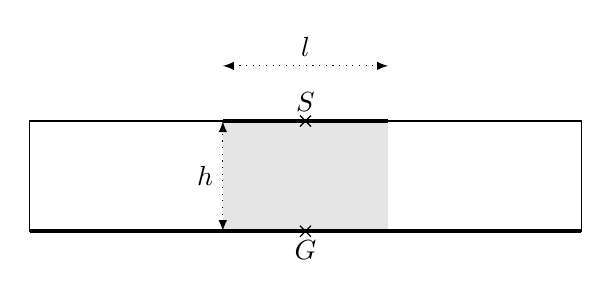
\begin{tikzpicture}[scale=7]
		\draw (0,0) rectangle (1,0.2);
		\fill[gray!20] (0.35,0) rectangle (0.65,0.2);
		\draw[-,ultra thick] (0,0) -- (1,0);
		\draw[-,ultra thick] (0.35,0.2) -- (0.65,0.2);
		\draw (0.5,0) node [below]{$G$};
		\draw[-] (0.49,-0.01) -- (0.51,0.01);
		\draw[-] (0.51,-0.01) -- (0.49,0.01);
		\draw (0.5,0.2) node [above]{$S$};
		\draw[-] (0.49,0.19) -- (0.51,0.21);
		\draw[-] (0.51,0.19) -- (0.49,0.21);
		\draw[dotted,arrows={latex-latex}]
			(0.35,0) -- node[midway,left]{$h$} (0.35,0.2);
		\draw[dotted,arrows={latex-latex}]
			(0.35,0.3) -- node[midway,above]{$l$} (0.65,0.3);
	\end{tikzpicture}
\end{figure}


La surface du générateur comprise entre la ligne microruban et le plan de masse
possède une impédance réelle dont la valeur est donnée par
la résistance $R_T$ du générateur de Thévenin :
\begin{align}
	z_s = \frac{l R_T}{h}.
\end{align}
Nous représentons cette impédance à l'aide du modèle de plaque mince
de Bérenger (section \ref{ssect:berenger}).

A cette impédance s'ajoute la tension $V_T$ entre les deux surfaces
métalliques de l'antenne représentées par le modèle PEC (section \ref{ssect:PEC}).
La direction du vecteur champ électrique appliqué entre ces deux bandes est donnée par :
\begin{align}
	\E_0 = \frac{\overrightarrow{GS}}{h l} ,
\end{align}
qui correspond à l'application d'une tension de $1$ V sur la surface,
puisque appliquée sur toute la largeur $l$.
Le champ électrique incident, tangeant à la surface, est alors donnée par :
\begin{align}
	\W_I = \Trp{\left(\frac{V_T}{R_T} \Trp{\E_0} , \Trp{0_{\Esp}}\right)} .
\end{align}
Nous injectons alors ce champ sur la surface à l'aide du flux non
dissipatif associé au modèle de Bérenger :
\begin{equation}
\FluxTHE{\W_\L}{\W_\R}{\n} = \FluxBER{\W_\L}{\W_\R + \W_I}{\n} .
\end{equation}
\\





\section{Permittivité et matériaux dispersifs}
\label{sect:permittivite}

La permittivité diélectrique $\EPrm$ d'un matériau présente dans les équations
de Maxwell influe sur la propagation d'une onde électromagnétique en affectant sa
vitesse de propagation et en causant un phénomène de réfraction-réflexion aux interfaces
entre deux matériaux de permittivité distincte. Dans le cas d'un matériau linéaire,
homogène, isotropique, et avec réponse instantanée, la permittivité peut être considéree
comme étant une constante réelle. C'est le cas dans le vide et, par convention, nous
noterons sa permittivité $\EPrm_0 = 8,854187 \cdot 10^{-12} \; \mathrm{F.m}^{-1}$. Mais de manière générale, la permittivité est fonction de
nombreux paramètres physiques comme la fréquence du champ électromagnétique considéré
ou bien la température et l'humidité du matériau.
\\

Les travaux de Gabriel \cite{Gabriel1,1996Gabiel,2009Gabriel} mettent en évidence l'influence de la fréquence
$\freq$ sur la permittivité des tissus humains dans la bande de 10 Hz à 20 GHz. Ces
travaux sont très intéressants en ce qui concerne les objets connectés qui rayonnent
généralement dans la bande des 1 à 3 GHz.


\begin{figure}[!h]
	\begin{center}
		\caption{
			\label{img:permittivites_variables}
			Permittivité relative de différents tissus humains
			sur la bande de fréquences de $1$ MHz à $10$ GHz.
			Données issues de la base de données IFAC-CNR.
		}
		
		\begin{tikzpicture}[scale=1]
		\begin{loglogaxis}[
		axis lines=middle,
		xlabel=$\freq$ (MHz), %x label style={anchor=north},
		ylabel=$\EPrm_r$,% y label style={at={(axis cs:0,-0.05)},anchor=east},
		xmin=1,xmax=25000,
		ymin=1,ymax=3500,
		%xtick={0,0.1,...,0.5},
		%ytick={0.999,1,1.001},
		%yticklabel style={/pgf/number format/.cd,fixed,precision=3},
		x post scale=1.5,
		y post scale=1.5,
		%legend style={at={(axis cs:1000,1.002)},anchor=north west}
		]
		
		\addplot[
		thick,
		mark=none,
		color=red,
		] table
		[x expr=\thisrowno{0}/1000000]
		{permittivites/heart.plt};
		\addlegendentry{Cœur}
		
		\addplot[
		thick,
		mark=none,
		color=blue,
		] table
		[x expr=\thisrowno{0}/1000000]
		{permittivites/brain.plt};
		\addlegendentry{Matière grise}
		
		\addplot[
		thick,
		mark=none,
		color=yellow,
		] table
		[x expr=\thisrowno{0}/1000000]
		{permittivites/fat.plt};
		\addlegendentry{Graisse}
		
		\addplot[
		thick,
		mark=none,
		color=green,
		] table
		[x expr=\thisrowno{0}/1000000]
		{permittivites/liver.plt};
		\addlegendentry{Foie}
		
		\addplot[
		thick,
		mark=none,
		color=pink,
		] table
		[x expr=\thisrowno{0}/1000000]
		{permittivites/muscle.plt};
		\addlegendentry{Muscle}

		\addplot[
		thick,
		mark=none,
		color=orange,
		] table
		[x expr=\thisrowno{0}/1000000]
		{permittivites/lung_empty.plt};
		\addlegendentry{Poumon (vide)}
		
		\addplot[
		thick,
		mark=none,
		color=orange,
		densely dashed,
		] table
		[x expr=\thisrowno{0}/1000000]
		{permittivites/lung_full.plt};
		\addlegendentry{Poumon (gonflé)}
		
		\end{loglogaxis}
		\end{tikzpicture}
	\end{center}
\end{figure}



Dans la suite, nous ferons référence à la permittivité relative
(figure \ref{img:permittivites_variables}) d'un matériau
$\Fn{\EPrm_r(f)}{\EnsR^{+}}{\EnsR^{+}}$ en fonction de
la permittivité absolue $\Fn{\EPrm(f)}{\EnsR^{+}}{\EnsR^{+}}$
dont l'expression est donnée par la formule :
\begin{align}
\EPrm_r = \frac{\EPrm}{\EPrm_0} .
\end{align}

\begin{remark}
	De manière analogue, la perméabilité magnétique relative $\HPrm_r$ d'un
	matériau est donnée en fonction de sa perméabilité absolue et de la perméabilité
	du vide
	$\HPrm_0 = 4 \pi \cdot 10^{-7} \; \mathrm{H.m}^{-1}$ par la formule :
	\begin{align}
	\HPrm_r = \frac{\HPrm}{\HPrm_0} .
	\end{align}
\end{remark}

\begin{remark}
	Si nous notons $\VL = 2.99792458 \cdot 10^{8} \; \mathrm{m.s}^{-1}$
	la vitesse de propagation d'une onde électromagnétique dans le vide, alors $\VL_r$,
	la vitesse de propagation dans un matériau diélectrique, est donné par :
	\begin{align}
	\VL_r = \frac{\VL}{\sqrt{\EPrm_r \HPrm_r}} .
	\end{align}
\end{remark}

%  PH: explique ce que tu veux faire: le CCPR arrive de nulle part
%\todo{expliquer pourquoi le modèle CCPR}
Le solveur \texttt{teta-clac} résoud les équations de Maxwell dans le domaine temporel.
Nous ne pouvons donc pas directement prendre en compte les permittivités
relatives dépendantes de la fréquence dans les calculs.
Ainsi, nous utilisons un modèle décomposant ces permittivités
en sommes de fractions rationnelles tel que les modèles SIBC
(section \ref{ssect:SIBC_plaque}) et BIBC (section \ref{ssect:bibc}).
Le modèle
\textit{Complex-Conjugate Poles-Residues} (CCPR) a été choisi \cite{ccpr_han,
ccpr_ramadan}. Il s'agit d'une généralisation des modèles de Debye
et Lorentz \cite{taflove2005computational}. L'expression du modèle CCPR est la suivante :
\begin{align}
\EPrm(\omega) = \EPrm_0 \EPrm_r(\omega) =
\EPrm_0 \EPrm_r^\infty + \EPrm_0
\sum_{k = 1}^{N_p} \frac{r_k}{j \omega - p_k} +
\frac{\overline{r_k}}{j \omega - \overline{p_k}}
\label{eq:ccpr_epsilon}
\end{align}
avec $\EPrm_r^\infty$ la permittivité
relative à la fréquence infinie, $N_p$ le nombre de pôles, $p_k \in \EnsC$
les pôles, $r_k \in \EnsC$ les résidus et $\overline{\lbrack.\rbrack}$ l'opérateur de
conjugaison complexe. Les pôles et résidus sont obtenus à l'aide de la technique du
\textit{vector fitting} \cite{772353} appliquée à la fonction
permittivité relative du matériau.


En écrivant l'équation de Maxwell-Ampère \eqref{eq:maxwell_ampere} dans le domaine
fréquentiel, nous avons :
\begin{align}
j \omega \EPrm(\omega) \tilde{\E} +
\ECnd \tilde{\E} - \Rot \tilde{\H} = 0 .
\end{align}
Puis, en substituant $\EPrm(\omega)$ dans cette équation par
l'expression du CCPR \eqref{eq:ccpr_epsilon}, nous obtenons :
\begin{align}
j \omega \EPrm_0 \left(\EPrm_r^\infty + 
\sum_{k = 1}^{N_p} \frac{r_k}{j \omega - p_k} +
\frac{\overline{r_k}}{j \omega - \overline{p_k}}\right)
\tilde{\E} + \ECnd \tilde{\E} - \Rot \tilde{\H} = 0 ,
\end{align}
soit encore :
\begin{align}
j \omega \EPrm_0 \EPrm_r^\infty \tilde{\E} + \left(\ECnd +
\EPrm_0 \sum_{k = 1}^{N_p} (r_k + \overline{r_k})\right) \tilde{\E} - \Rot
\tilde{\H} = - \sum_{k = 1}^{N_p} (\tilde{\J}_k + \tilde{\J}'_k)
\label{eq:ccpr_ampere}
\end{align}
avec, pour $k \in \Range{1}{N_p}$ :
\begin{align}
\tilde{\J}_k = \frac{\EPrm_0 r_k p_k}{j \omega - p_k} \tilde{\E} ,
\; \mathrm{et} \;
\tilde{\J}'_k = \frac{\EPrm_0 \overline{r_k} \overline{p_k}}{j \omega - \overline{p_k}} \tilde{\E}
\label{eq:ccpr_courants} .
\end{align}

En réécrivant les équations \eqref{eq:ccpr_ampere} et \eqref{eq:ccpr_courants}
dans le domaine temporel (par transformée de Fourier-Laplace inverse), et
en remarquant que les champs électromagnétiques sont toujours réels
(les courants annexes $\J_k$ et $\J'_k$ vérifient $\J_k = \J'_k$),
nous obtenons après calculs le système différentiel suivant :
\begin{subequations}
	\begin{align}
	\Ptl{t} \EPrm_0 \EPrm_r^\infty \E + (\ECnd +
	2 \EPrm_0 \sum_{k = 1}^{N_p} \Re(r_k)) \E - \Rot
	\H &= - 2 \sum_{k = 1}^{N_p} \Re(\J_k) ,
	\\
	\Ptl{t} \J_k - p_k \J_k - \EPrm_0 r_k p_k \E &= 0, \; \mathrm{pour} \;
	k \in \Range{1}{N_p} ,
	\end{align}
\end{subequations}
avec $\Re$ la fonction partie réelle.

Nous obtenons alors un couplage entre le schéma GD et $N_p$
courants vectoriels complexes annexes vérifiant chacun une
équation différentielle ordinaire.
Ce modèle est bien défini et stable si les parties réelles des pôles $p_k$
sont négatives.
\\



\section*{Conclusion}


Dans ce second chapitre, nous avons présenté plusieurs modèles de simulation.
Nous avons commencé par décrire des modèles de conditions de bord respectant la
condition de décroissance de l'énergie associée à la solution
assurant l'existence de la solution.
Nous avons aussi présenté la construction d'une condition aux limites
simulant un domaine infini par l'adjonction d'un domaine englobant
sur lequel les équations de Maxwell sont résolues dans l'espace complexe.
Ce problème complexe est aussi un système de Friedrichs.

Ensuite, nous avons énuméré un ensemble de modèles permettant de simuler
les plaques minces de matériaux. Ces modèles permettent de remplacer
les volumes fins par des surfaces et sont complémentaires sur une
large bande de fréquences.
Le remplacement des mailles fines par des surfaces va nous permettre
de réduire les temps de simulation et faciliter les phases de maillage.

Nous avons aussi présenté des modèles permettant d'injecter
un signal dans la scène simulée, notamment utilisé dans les
simulations faisant intervenir une antenne.

Enfin, dans le but de traiter les matériaux diélectriques dont la permittivité
varie en fonction de la fréquence, nous avons donné un modèle volumique prenant
en compte ces variations.
\\

Dans le chapitre suivant,
nous décrivons une implémentation sur mailles hexaédriques 
de la formulation semi-discrète présentée au chapitre \ref{chap:generalites}.
Cette implémentation a nécessité le choix d'un espace d'approximation
dont nous décrivons les propriétés et les simplifications qu'elles induisent.



















